\usetikzlibrary{arrows.meta}
\tikzset{%
  >={Latex[width=2mm,length=2mm]},
  % Specifications for style of nodes:
            minerbase/.style = {rectangle,
                           minimum width=3cm, minimum height=1cm,
                           text centered, font=\stfamily},
            base/.style = {rectangle, rounded corners, draw=black,
                           minimum width=3cm, minimum height=1cm,
                           text centered, font=\sffamily},
  censoredminer/.style = {minerbase, draw=red!30},
  uncensoredminer/.style = {minerbase, draw=blue!30},
  majority/.style = {base, fill=blue!30},
  minority/.style = {base, fill=red!30},
    common/.style = {base, fill=green!30},
 blacklist/.style = {base, minimum width=2cm, fill=orange!70}
}

\subsection{Expected Results}
In addition to designing experiments to test how the bitcoind client behaves, we also analyzed its source code. According to the source code, if a client is told that a block exists, but is unable to get a copy of that block and validate it, the client will continue assuming the last head of the blockchain it validated is the current head\footnote{Specifically, line 2668 validation.cpp in bitcoind version 0.14: https://github.com/bitcoin/bitcoin/blob/0.14/src/validation.cpp#L2668}. In the scenario we consider, the censored client would be able to recieve a message from non-censored clients telling it that a new block exists. But when the client then requested the contents of the block from the non-censored clients, the respone containing the new block's data would would never be recieved. From the point of view of the censored client, this is indistingushable from a miner broadcasting headers but not sending the full block data. The source code for bitcoind explicitly describes such an attack and contains logic to ensure, in this scenario, the block is not added to a client's index.

\begin{figure}[h]
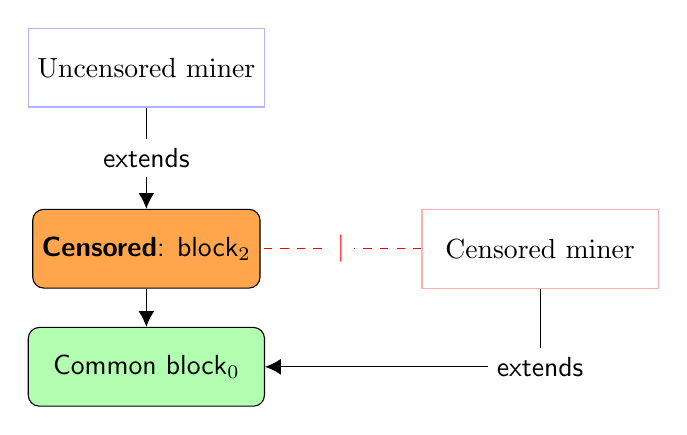
\begin{tikzpicture}[every node/.style={node distance=1.5cm,fill=white, font=\sffamily}, align=center]
  %\node (majority2)[majority, above of=majority1] {Majority block};
  \node (bad)   [blacklist]                {\textbf{Censored}: block$_2$};

  \node (fmine)[uncensoredminer, above of=bad, yshift=.8cm] {Uncensored miner};
  \node (cmine)[censoredminer, right of=bad, xshift=3.5cm] {Censored miner};
  \node (start)  [common, below of=bad]    {Common block$_0$};

    \draw[->]             (bad) -- (start);
    \draw[->]             (fmine) -- node{extends} (bad);
    \draw[->]             (cmine) |- node{extends} (start);
    \draw[red,dashed]             (cmine) --node{$|$} (bad);
\end{tikzpicture}
\caption{After a censored block is mined, miners try extending different blocks}
\end{figure}

\subsubsection{Censored minority % TODO the figures aren't going in the sections because we don't have enough text around them}
\begin{figure}[h]
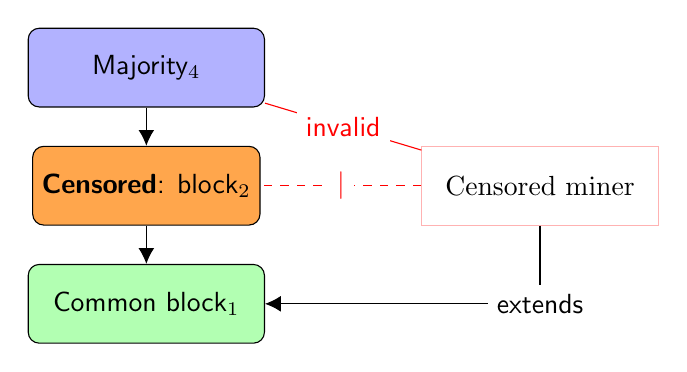
\begin{tikzpicture}[every node/.style={node distance=1.5cm,fill=white, font=\sffamily}, align=center]
  %\node (majority2)[majority, above of=majority1] {Majority block};

  \node (bad)   [blacklist]                {\textbf{Censored}: block$_2$};
  \node (start)  [common, below of=bad]    {Common block$_1$};
  \node (majority1)[majority, above of=bad] {Majority$_4$};
  \node (miner)[censoredminer, right of=bad, xshift=3.5cm] {Censored miner};

    \draw[red]          (miner) -- node{invalid} (majority1);
    \draw[red,dashed]     (miner) -- node{$|$} (bad);
    \draw[->]             (miner) |- node{extends} (start);
    \draw[->]             (majority1) -- (bad);
    \draw[->]             (bad) -- (start);
\end{tikzpicture}
\caption{Censored minors will see future blocks added by uncensored miners, but will not be able to validate their chain so they will be ignored}
\end{figure}

% TODO the figures aren't going in the sections because we don't have enough text around them
\subsubsection{Censored majority}

\begin{figure}[h]
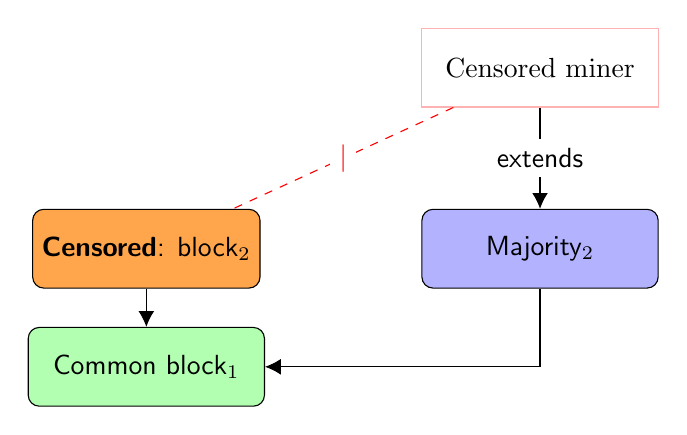
\begin{tikzpicture}[every node/.style={node distance=1.5cm,fill=white, font=\sffamily}, align=center]
  %\node (majority2)[majority, above of=majority1] {Majority block};

  \node (bad)   [blacklist]                {\textbf{Censored}: block$_2$};
  \node (start)  [common, below of=bad]    {Common block$_1$};
  \node (majority1)[majority, right of=bad, xshift=3.5cm] {Majority$_2$};
  \node (miner)[censoredminer, above of=majority1, yshift=.8cm] {Censored miner};

    \draw[->]          (miner) -- node{extends} (majority1);
    \draw[red,dashed]     (miner) -- node{$|$} (bad);
    \draw[->]             (majority1) |- (start);
    \draw[->]             (bad) -- (start);
\end{tikzpicture}
\caption{If censored miners mine faster than uncensored miners, the two forks will eventually grow to be of equal length}
\end{figure}

\begin{figure}[h]
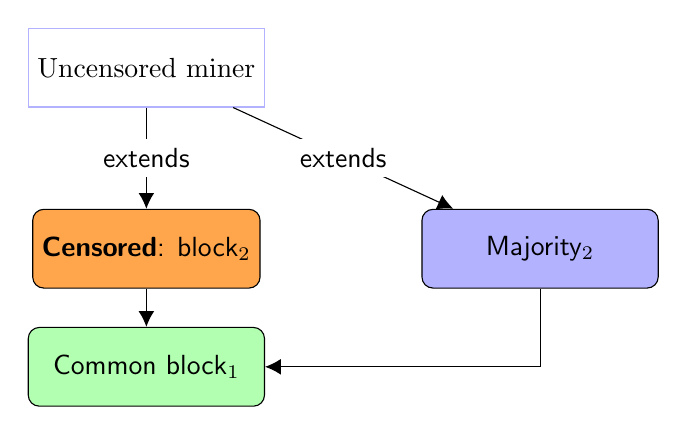
\begin{tikzpicture}[every node/.style={node distance=1.5cm,fill=white, font=\sffamily}, align=center]
  %\node (majority2)[majority, above of=majority1] {Majority block};

  \node (bad)   [blacklist]                {\textbf{Censored}: block$_2$};
  \node (start)  [common, below of=bad]    {Common block$_1$};
  \node (majority1)[majority, right of=bad, xshift=3.5cm] {Majority$_2$};
  \node (miner)[uncensoredminer, above of=bad, yshift=.8cm] {Uncensored miner};

    \draw[->]          (miner) -- node{extends} (majority1);
    \draw[->]     (miner) -- node{extends} (bad);
    \draw[->]             (majority1) |- (start);
    \draw[->]             (bad) -- (start);
\end{tikzpicture}
\caption{Uncensored miners can mine off of either block when the forked chains are of equal length}
\end{figure}

\begin{figure}[h]
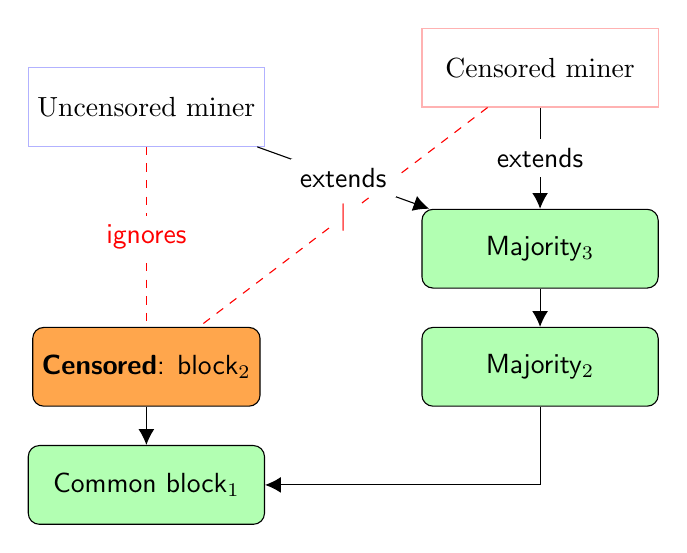
\begin{tikzpicture}[every node/.style={node distance=1.5cm,fill=white, font=\sffamily}, align=center]
  %\node (majority2)[majority, above of=majority1] {Majority block};

  \node (bad)   [blacklist]                {\textbf{Censored}: block$_2$};
  \node (start)  [common, below of=bad]    {Common block$_1$};
  \node (majority1)[common, right of=bad, xshift=3.5cm] {Majority$_2$};
  \node (majority2)[common, above of=majority1] {Majority$_3$};
  \node (cminer)[censoredminer, above of=majority2, yshift=.8cm] {Censored miner};
  \node (fminer)[uncensoredminer, above of=bad, yshift=1.8cm] {Uncensored miner};

    \draw[red,dashed]     (cminer) -- node{$|$} (bad);
    \draw[red,dashed]     (fminer) -- node{ignores} (bad);
    \draw[->]     (cminer) --node{extends} (majority2);
    \draw[->]     (fminer) --node{extends} (majority2);
    \draw[->]             (majority1) |- (start);
    \draw[->]             (bad) -- (start);
    \draw[->]             (majority2) -- (majority1);
\end{tikzpicture}
\caption{Since the majority of mining power is mining off one fork, that fork will eventually grow to be longer than the other and all miners will agree on it }
\end{figure}
